\subsection{Distance controller}\label{ssec:distanceController}
A distance controller will now be designed, to complement the directional controller.
As concluded in \secref{sec:SteeringModel}, a deviation from the planned line, will cause the vehicle to drive at a parallel line, beside the planned line. The deviation will be calculated from the position provided by the GoT system. As the deviation is a function of the error angle integrated over time, it is assumed that a P controller will be sufficient to handle this function, just as in the Angular controller. The controller will therefore be based on a P controller, and iterated until results are satisfactory. 

As real-world test data is not available, caused by the magnetometer not working in the room with the GoT system installed, the controller will be designed and simulated in Simulink. As a starting point, the proportional gain will be set at 1, and the controller will be designed based on bode plots and step responses.

The proposed controlling scheme can be seen in \figref{SteeringSimulink}

\begin{figure}[H]
\centering
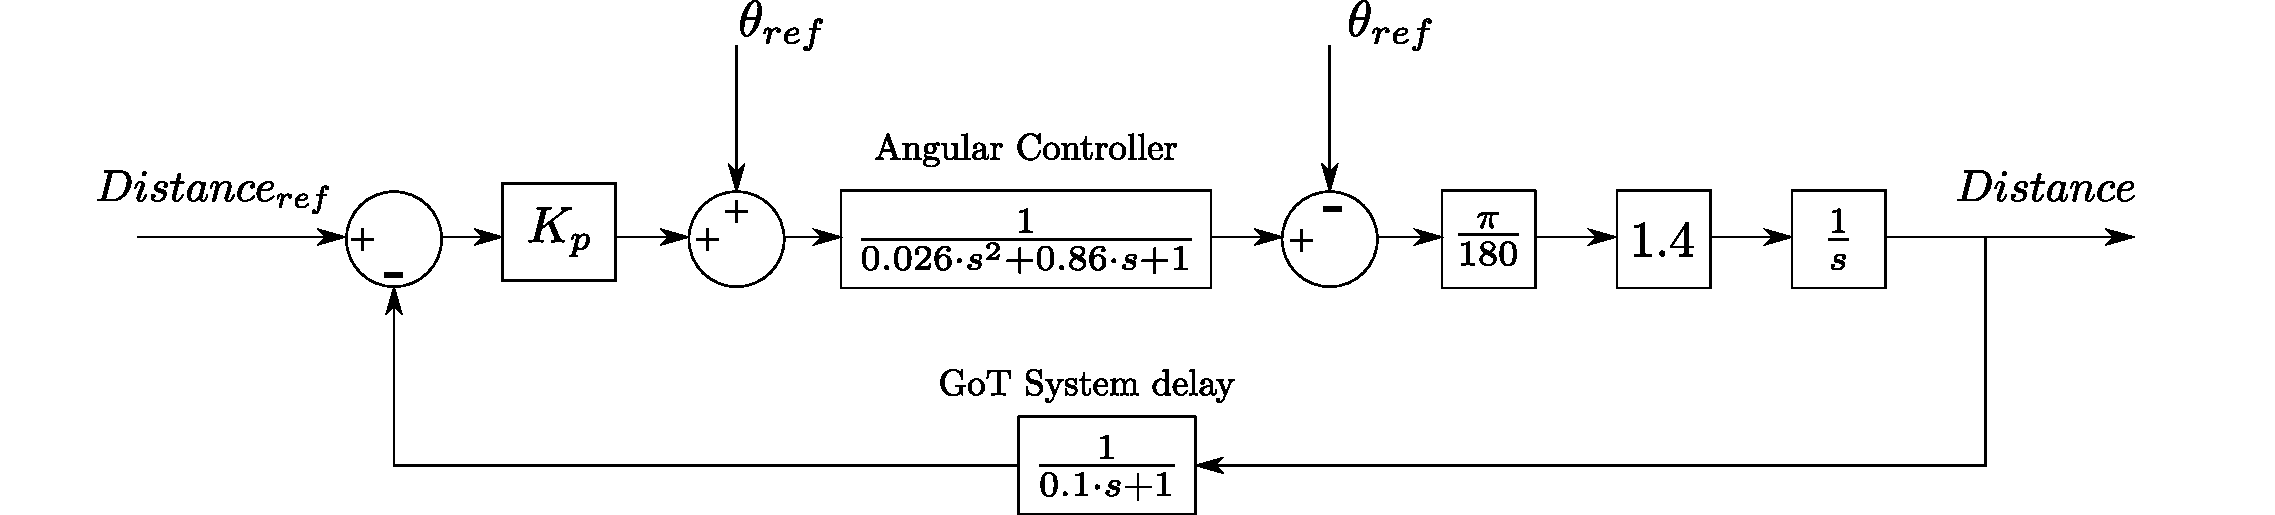
\includegraphics[width=1.1\textwidth]{figures/steeringFullModel.pdf} 
\caption{Initial Distance Controller}
\label{SteeringSimulink}
\end{figure}

As illustrated in the figure, the directional controller is located in the center of the loop, as this will be responsible for changing the vehicle's angle, to what the distance loop calculates to be necessary. A reference angle, \emph{angleRef} is added to the output of the P controller, representing the angle of the line to follow. To prevent the P controller from over-regulating, and command the system to turn, e.g. 360 degrees, it is limited by a floor and ceiling of $\pm 90^\circ$. The following three stages (Deg to radians, Velocity and Deviation integrator) are taken directly from the steering model \figref{fig:steeringLineFollowingModel}.

According to \secref{GoTSystem}, the GoT system provides position updates every 100ms. To model this delay, the same approximation as used for the servo delay in \secref{directionalExtention}, will be implemented:
$$\frac{1}{\lambda\cdot\text{s}+1}\Rightarrow\frac{1}{\SI{0,1}\cdot\text{s}+1}
$$
The input to the loop is the wanted deviation from the line. This should ideally be zero, but is set to 1m in the simulation. This is done, to avoid an initial error, when simulation the controller. The error integrator starts at zero when the simulation is started, so a input of zero would imply that the vehicle is not deviating from the route and therefore no error. Since the system is assumed linear, a step from 1m to 0m error, should be the same as the opposite and therefore can the simulation be utilized this way. The resulting step response can be seen in \figref{SimulationSteeringP1}

\begin{figure}[H]
  \centering
 	%Trim margins @:   left        bottom       right       top
 	\adjustbox{ trim = {.15\width} {.30\height} {.15\width} {.30\height}, clip }
  {
    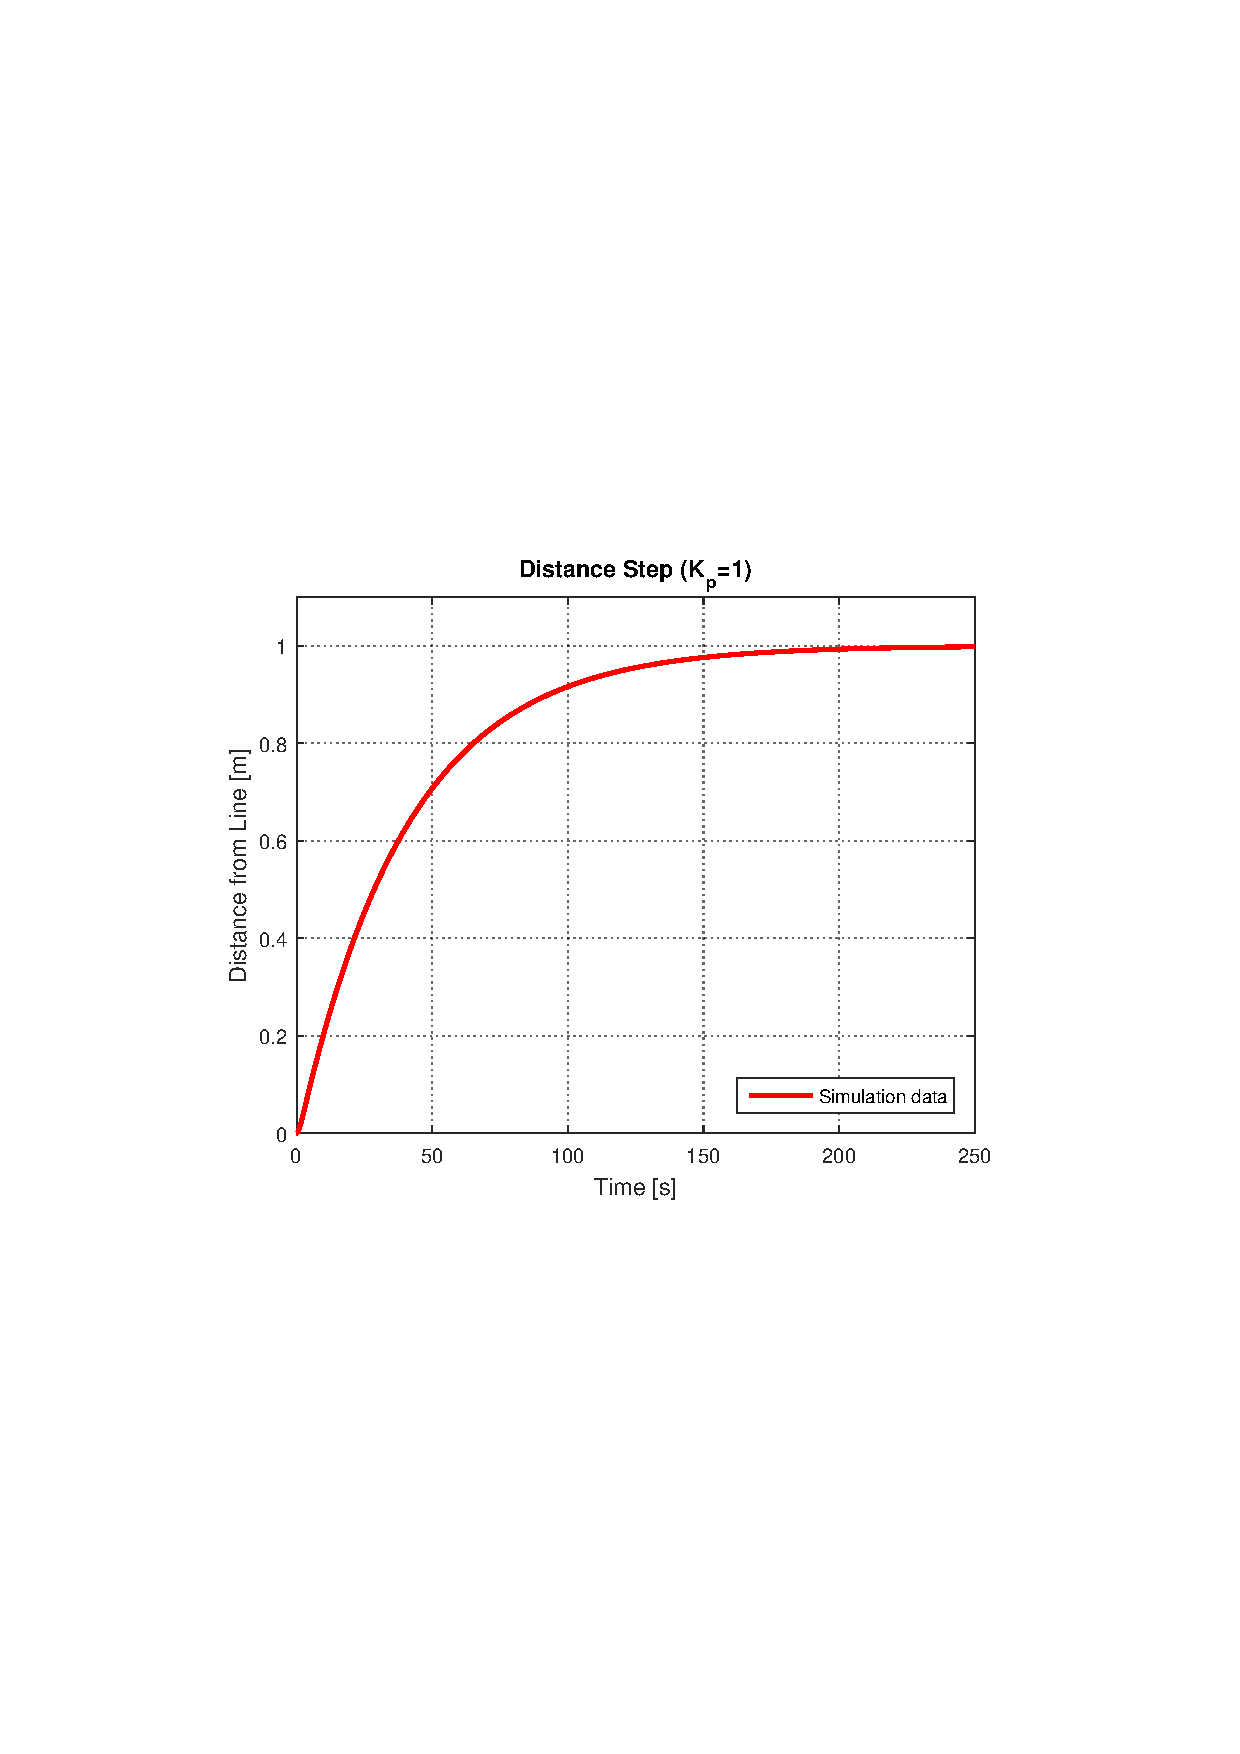
\includegraphics[width=1.4\textwidth]{figures/distanceStep1.pdf}
  }
  \caption{A simulated step-response of the system correcting a 1 meter offset}
  \label{SimulationSteeringP1}
\end{figure}
As seen on \figref{SimulationSteeringP1}, the system takes around 240 seconds, i.e. 4 minutes, to correct the error, which leaves room for improvements.

Using the Linear Analysis function of Simulink, a Bode plot is made from the open loop system. The resulting plot can be seen in \figref{SimulationSteeringB1}
\begin{figure}[H]
  \centering
 	%Trim margins @:   left        bottom       right       top
 	\adjustbox{ trim = {.15\width} {.30\height} {.15\width} {.30\height}, clip }
  {
    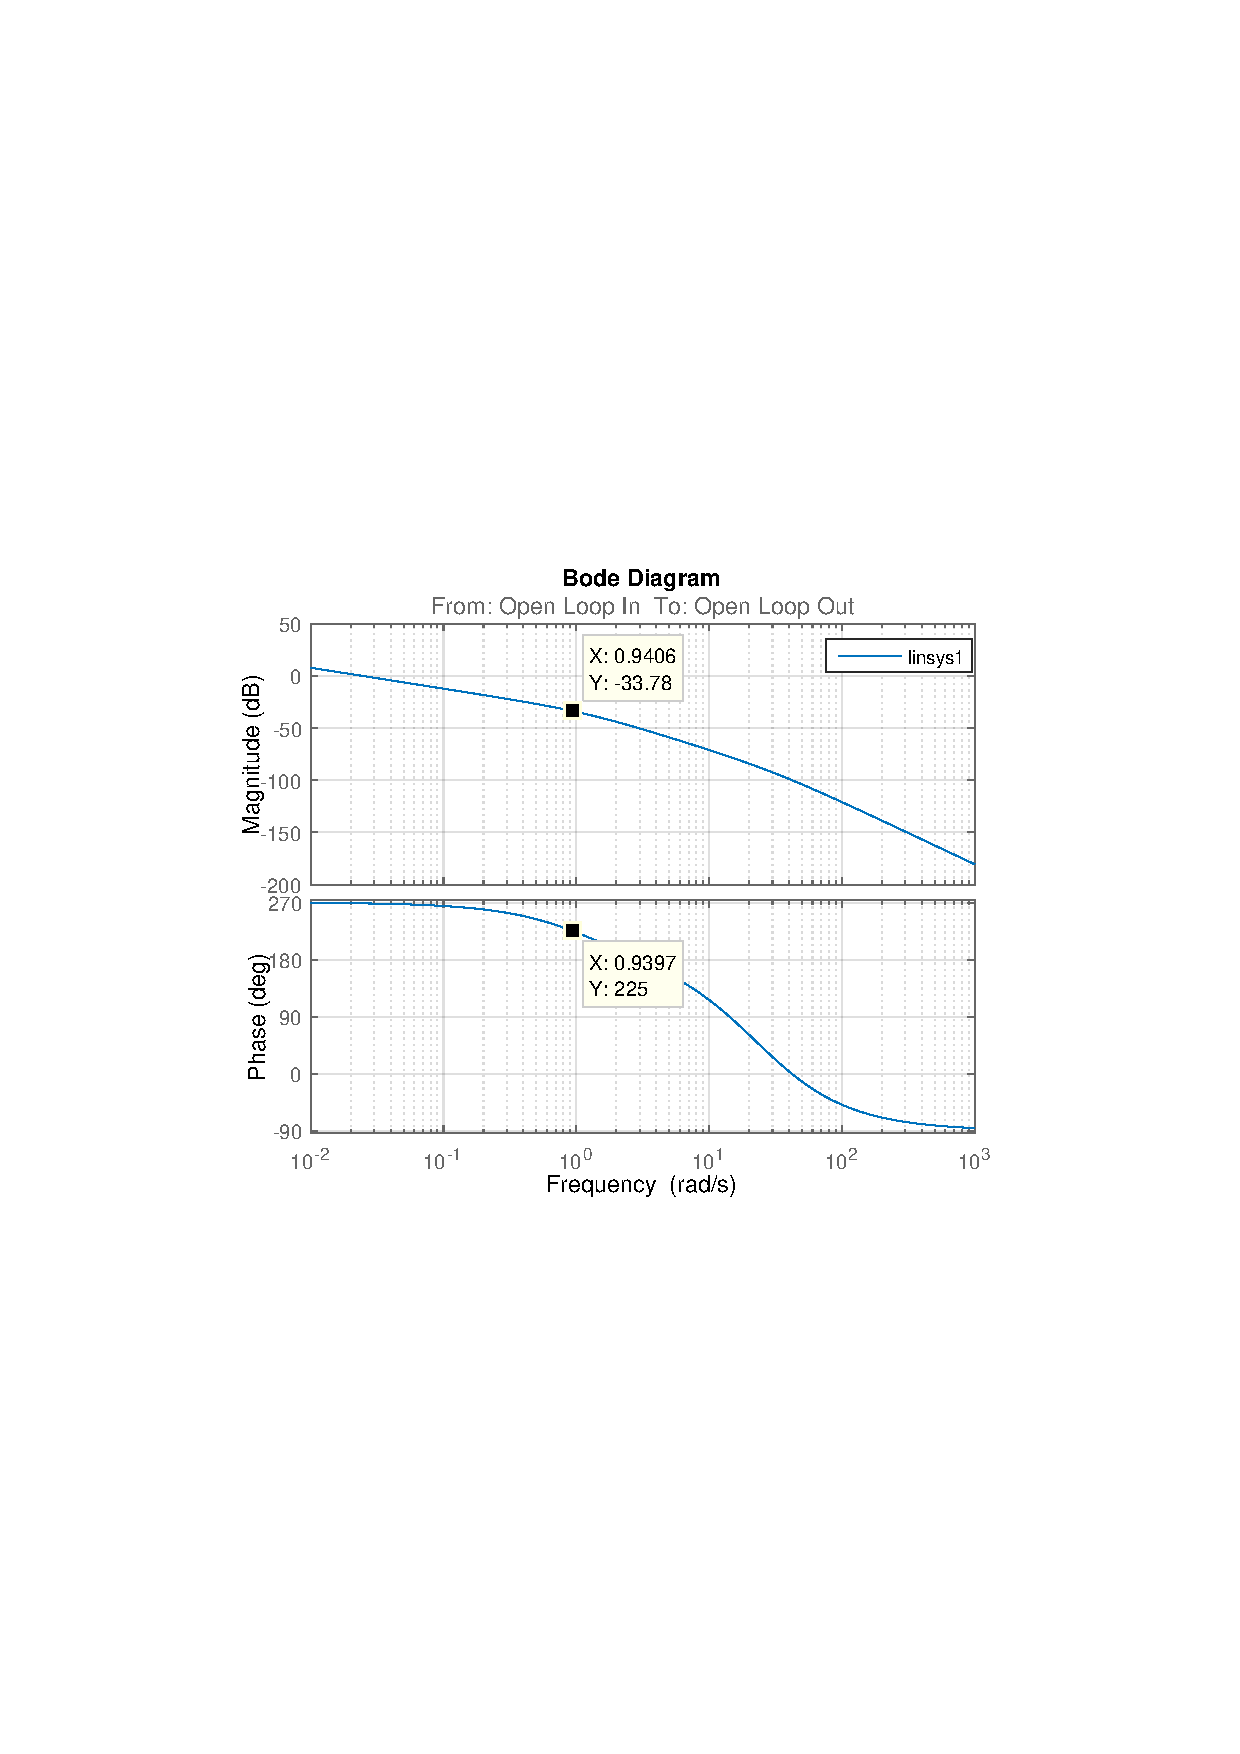
\includegraphics[width=1.4\textwidth]{figures/distanceBode1.pdf}
  }
  \caption{An open loop Bode plot of the system with a $K_p$ on 1.}
  \label{SimulationSteeringB1}
\end{figure}

To improve the system response, the $K_p$ value is changed. This is done by looking at the phase margin. As a system with phase margin on 45 degrees will give a stable system, with the highest gain, the $K_p$ is set to give this phase margin. As seen on \figref{SimulationSteeringB1}, the gain is \SI{-33,78}dB at the 45 degree point (225-45=180). To get 0 dB gain at this point, the proportional gain will be increased by  \SI{33,78}dB:
$$\text{K}_\text{p}=10^{\frac{\SI{33,78}{}}{20}} = \SI{48,87}{}$$

The new value is used and yields the step response illustrated in \figref{SimulationSteeringP2}.

\begin{figure}[H]
  \centering
 	%Trim margins @:   left        bottom       right       top
 	\adjustbox{ trim = {.15\width} {.30\height} {.15\width} {.30\height}, clip }
  {
    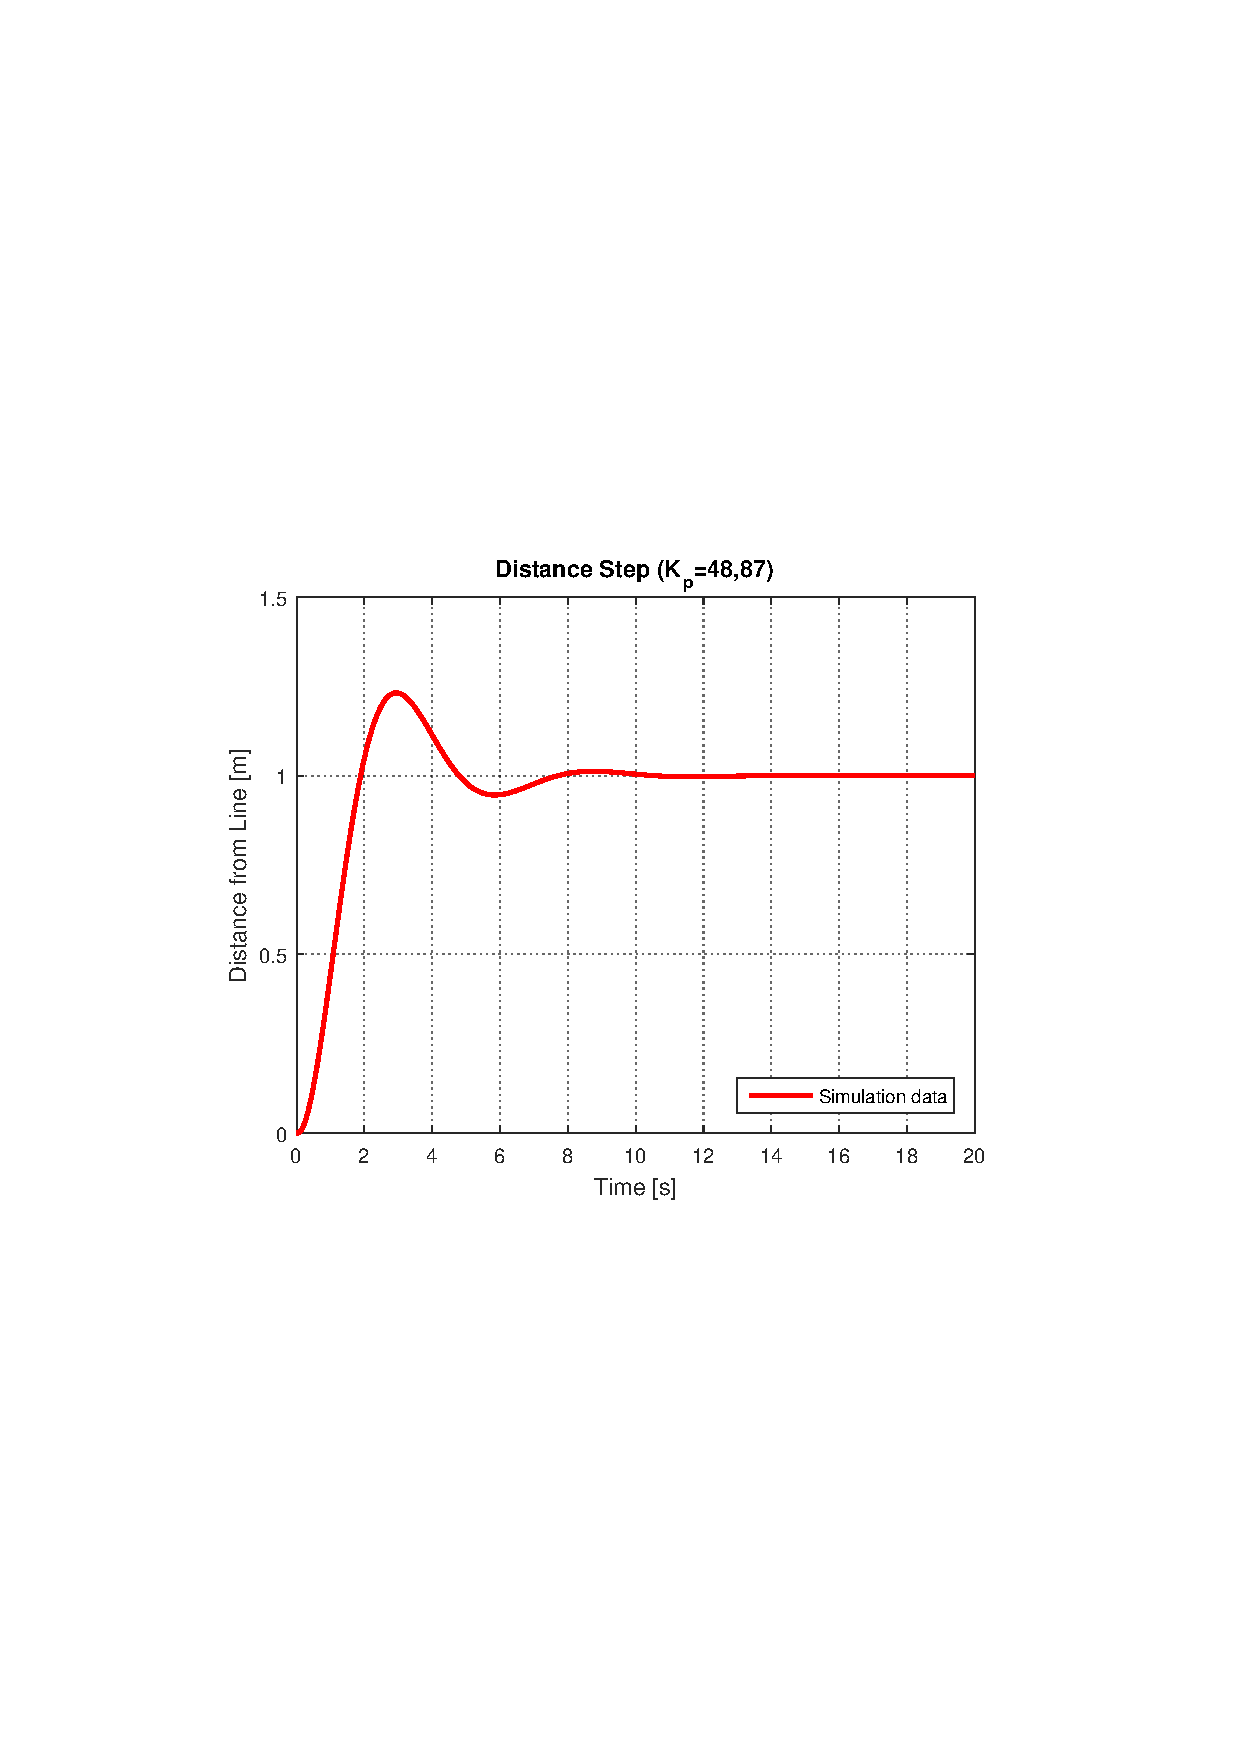
\includegraphics[width=1.4\textwidth]{figures/distanceStep2.pdf}
  }
  \caption{Step response with new $\text{K}_\text{p}$ on 48,87.}
  \label{SimulationSteeringP2}
\end{figure}
As seen on \figref{SimulationSteeringP2}, the response has improved and the system reaches the target in approximately 2 seconds. The higher $K_p$ gives overshoots and rings, that first settles after 10 seconds. It is improved, when compared to the response on \figref{SimulationSteeringP1}, but still needs improvements. If the overshoot is removed, the settling time will be around 2 seconds. A way to remove an overshoot is to increase the high frequency gain \cite{KMNielsen}. This can be done by adding a differentiator to the controller, which will then become a PD controller. According to \cite{Franklin}, a PD controller is rarely used in real life, as it is extremely sensitive to noise, and a lead compensator is recommended instead.
%
\begin{flalign}
  \eq{K_{lead}}{\frac{1 + a \cdot s}{1 + b \cdot s}}\label{eq:DCeq1}
\end{flalign}
%
A lead compensator, see \eqref{eq:DCeq1}, adds a zero to the system, which cancels out one of the poles in the system. This lowers the phase shift, improving the phase margin, and increases the gain at higher frequencies. At the same time, a pole is added at an even higher frequency, in order to ensure stability in the system.

The sampling period of the loop is limited to 100ms by the GoT system. According to the Nyquist-Shannon sampling theorem, a signal needs to be sampled by at least twice the signal bandwidth. This limits the upper frequency of which the pole in the lead compensator can be placed. To ensure the theorem is fulfilled, the pole is given a time constant of \SI{0,3}{s}. This in turn limits the frequency of the zero - if the zero is placed too close to the pole, they will cancel each other out. On the other hand, it is desired to place the zero as high as possible, in order to not change the low frequency gain, and at the same time to affect the existing poles in the system as much as possible. A compromise must be made, and the zero is given a time constant of 1 second. This yields a new controller layout, which can be seen on \figref{FinalDist}.

\begin{figure}[H]
  \centering
    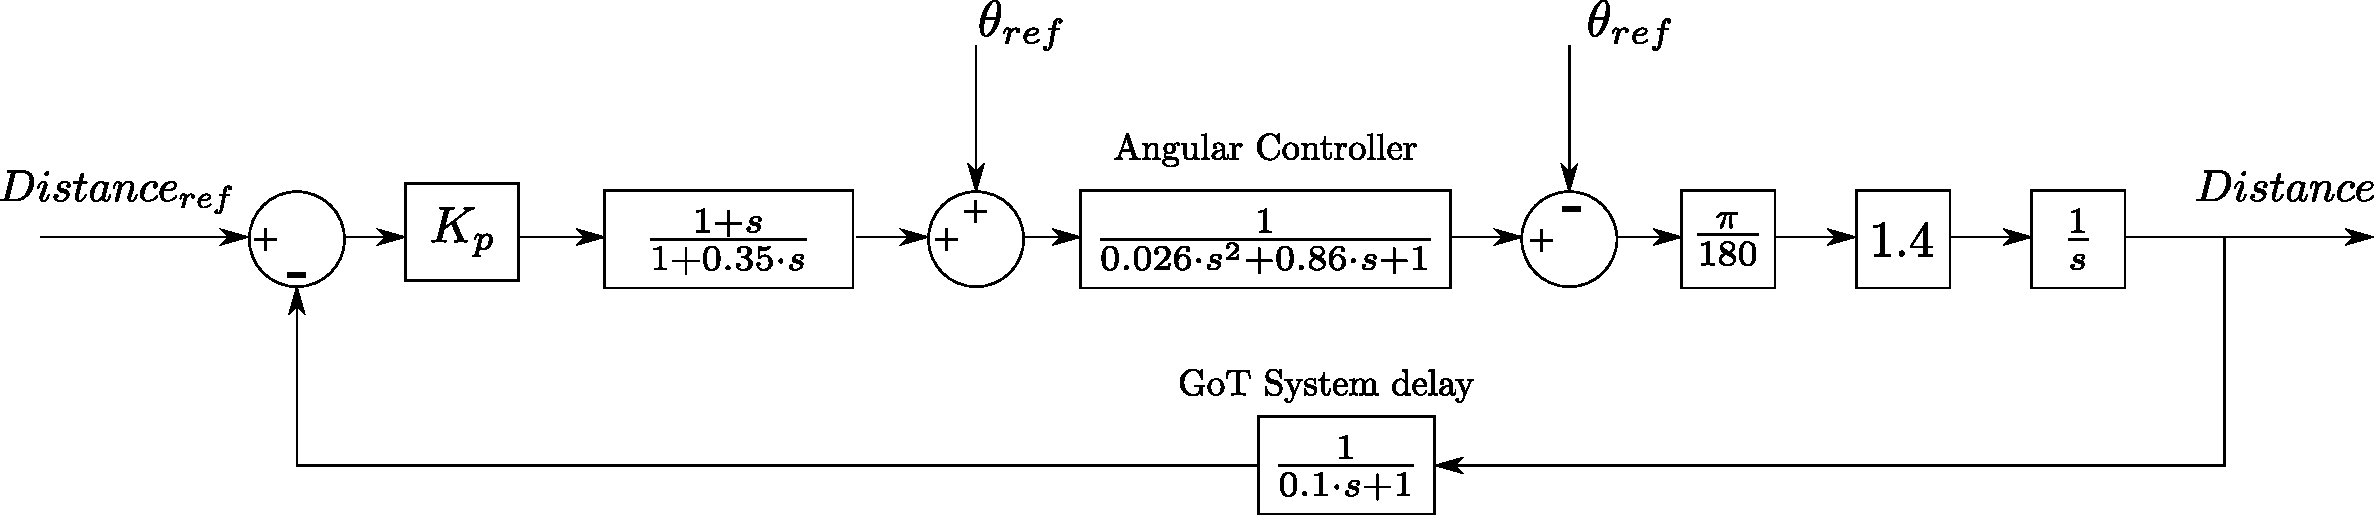
\includegraphics[width=\textwidth]{figures/finalDistanceController.pdf}
  \caption{Distance controller with lead compensator}
  \label{FinalDist}
\end{figure}

A bode plot is made with the lead compensator added to the system, shown on \figref{SimulationSteeringB2}. 

\begin{figure}[H]
  \centering
 	%Trim margins @:   left        bottom       right       top
 	\adjustbox{ trim = {.15\width} {.30\height} {.15\width} {.30\height}, clip }
  {
    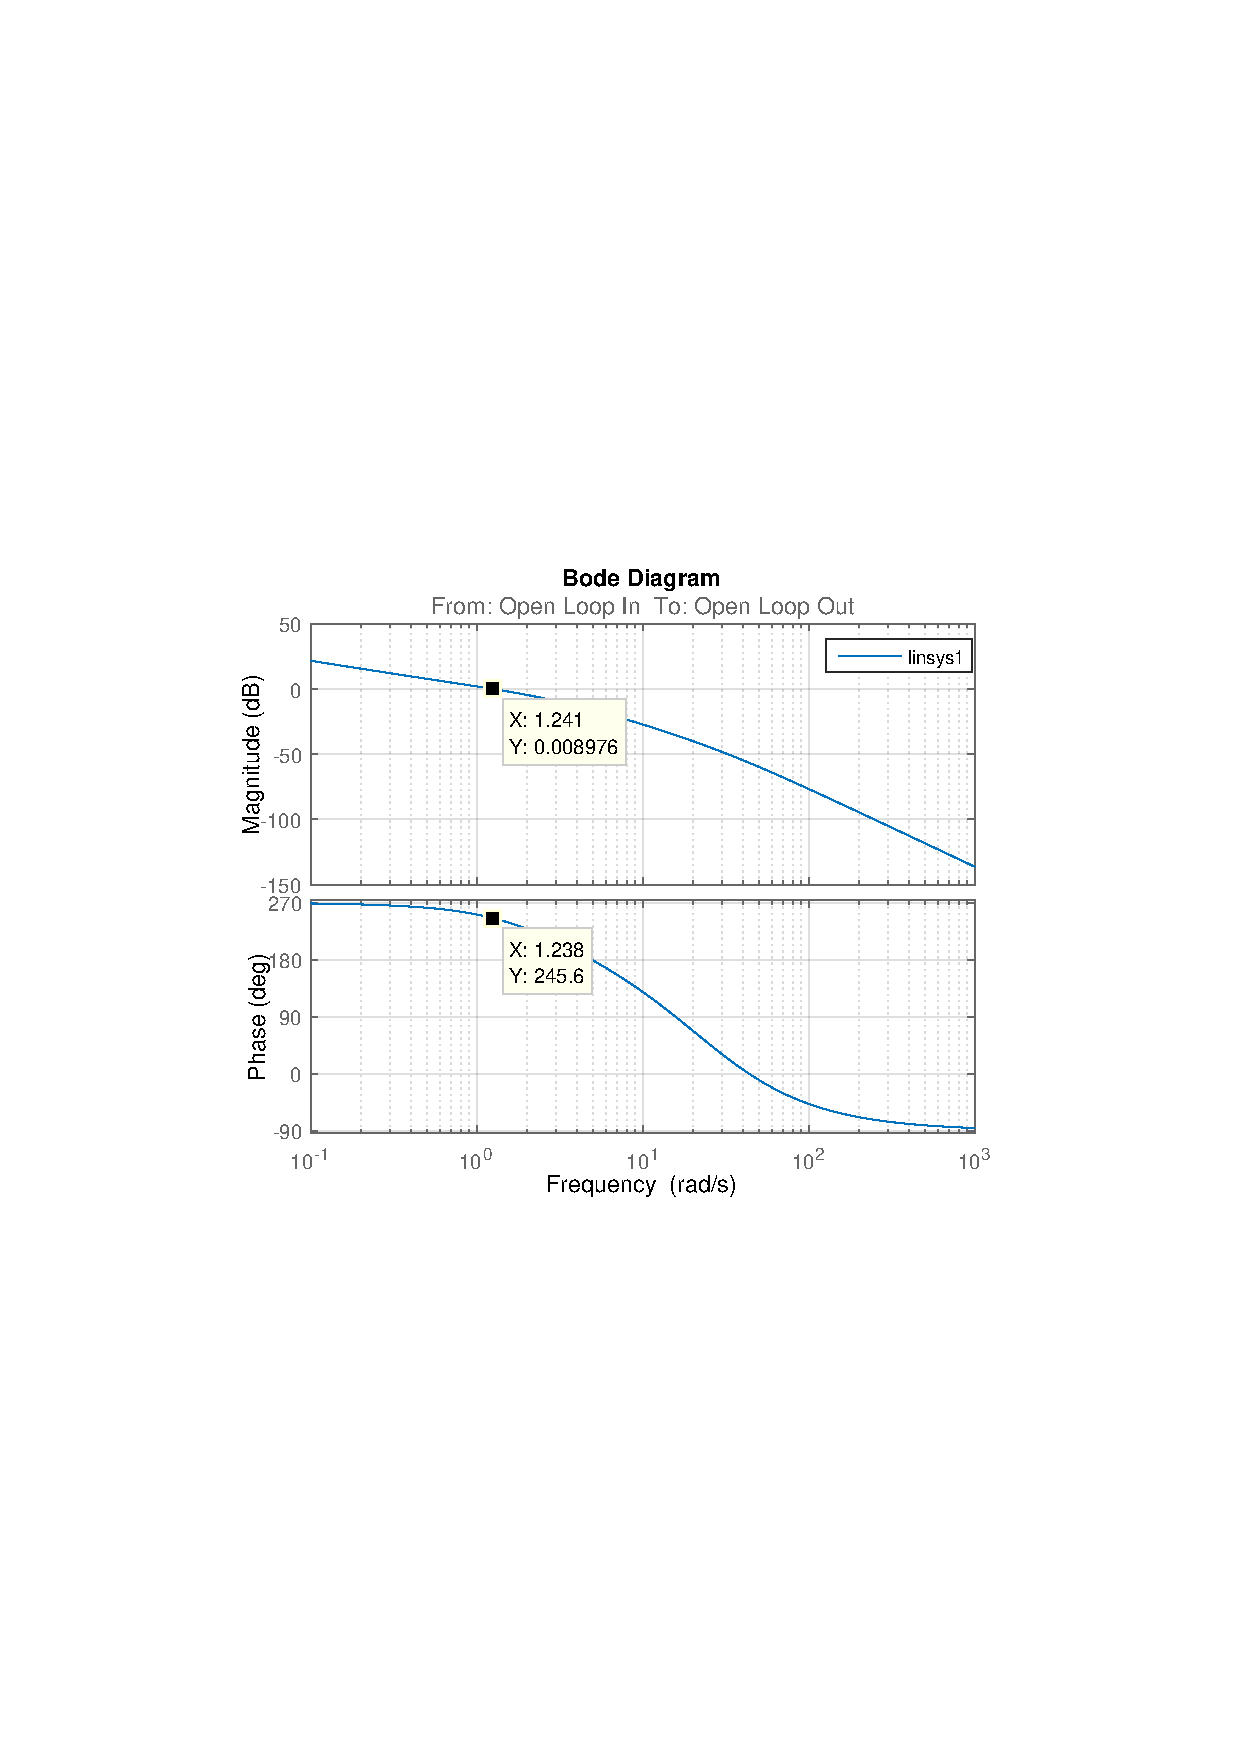
\includegraphics[width=1.4\textwidth]{figures/distanceBode2.pdf}
  }
  \caption{Bodeplot with lead compensation}
  \label{SimulationSteeringB2}
\end{figure}
The 0 dB frequency has increased from 0,94 \si{\frac{rad}{s}} to 1,24 \si{\frac{rad}{s}}, and the phase margin is now: $$\SI{245,6}{}-180=\SI{65,6}{^\circ}$$

The lead compensator has increased the gain at higher frequencies and improved the phase margin. That is made a new step response for the controller with lead compensator, shown on \figref{SimulationSteeringP3}.

\begin{figure}[H]
  \centering
 	%Trim margins @:   left        bottom       right       top
 	\adjustbox{ trim = {.15\width} {.30\height} {.15\width} {.30\height}, clip }
  {
    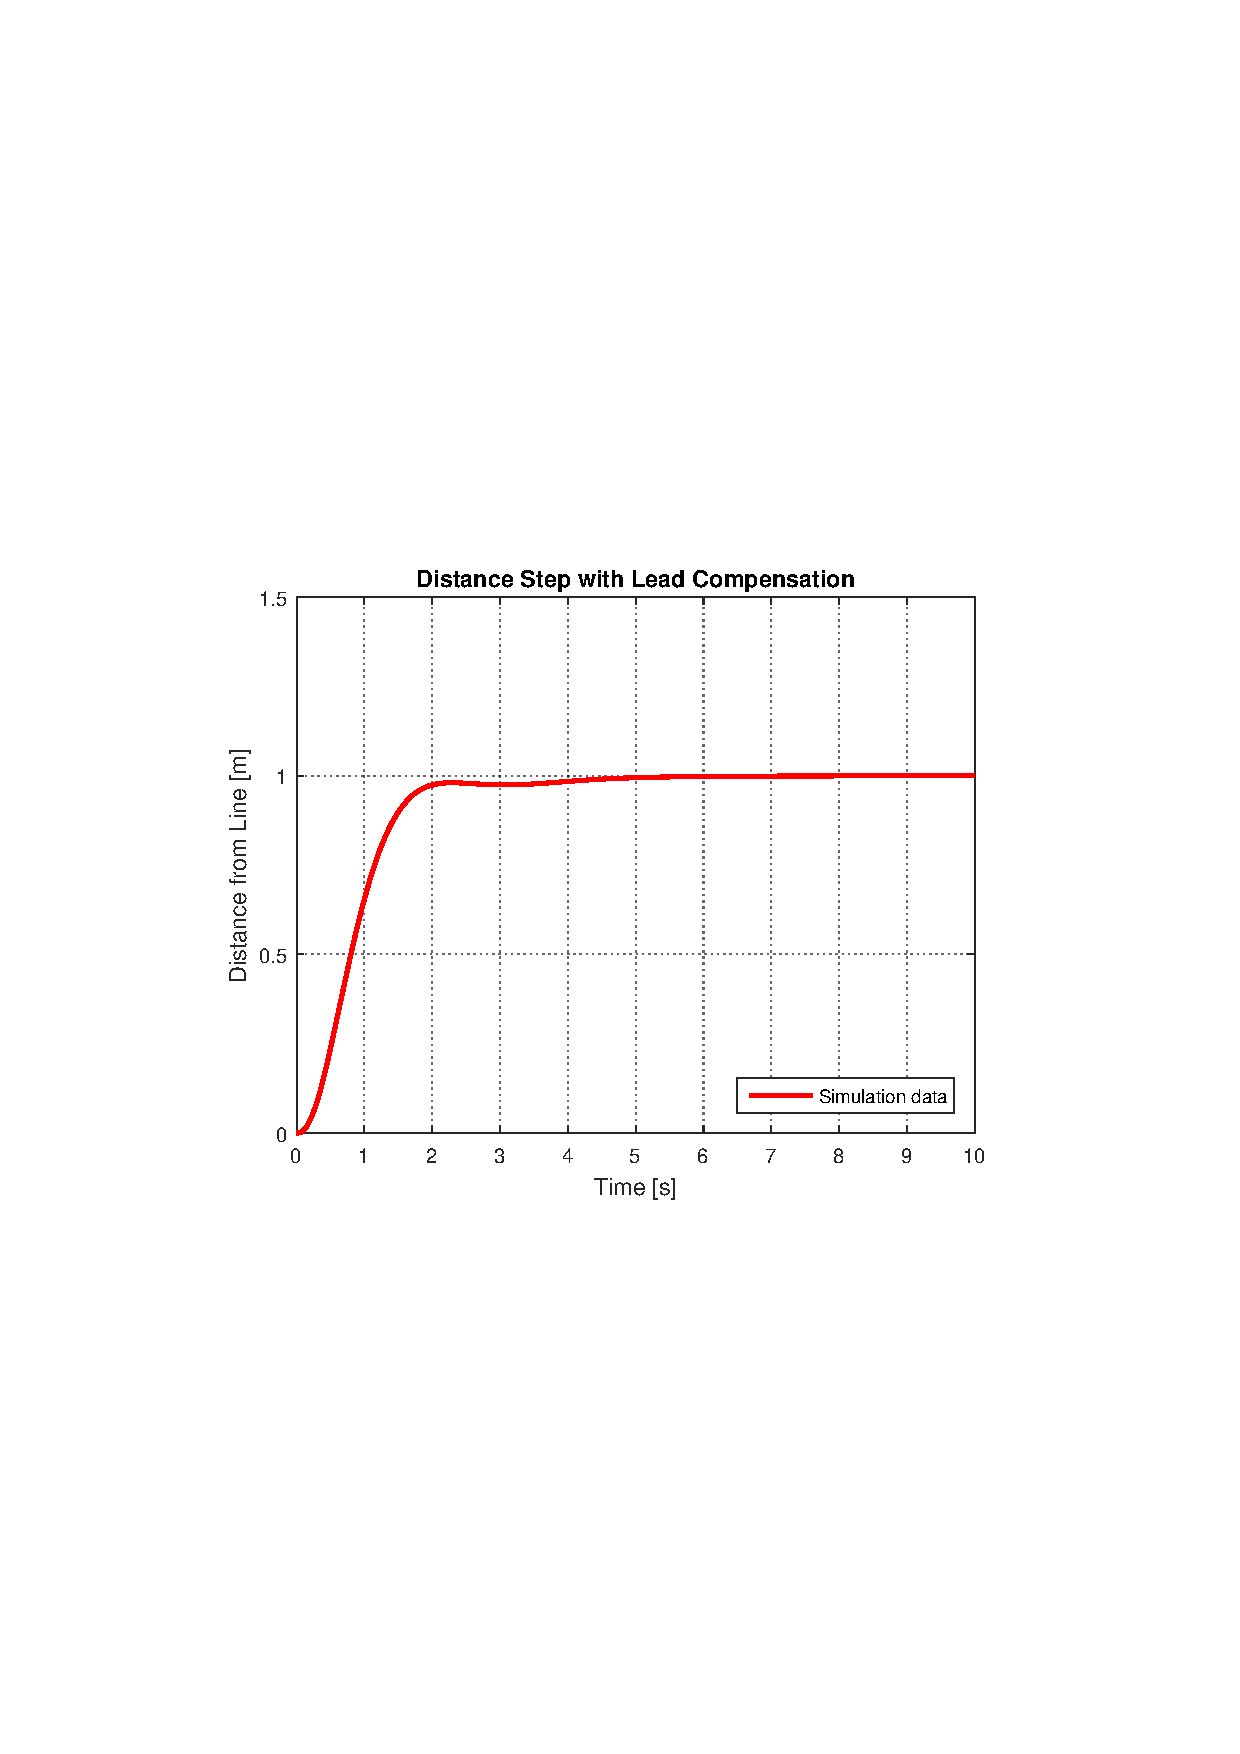
\includegraphics[width=1.4\textwidth]{figures/distanceStep3.pdf}
  }
  \caption{Step response with lead compensation}
  \label{SimulationSteeringP3}
\end{figure}
As seen on \figref{SimulationSteeringP3}, the system reaches the target in approximately two seconds, and the ringing has been reduced to less than \SI{3}{cm}. This is considered acceptable and the gain is not changed, to get a phase margin on 45 degrees. It is desirable to keep the increased phase margin. As the whole loop is based on an approximated model, with no real data to verify it. The extra phase margin will provide a better chance of a stable system in the real world.